\section{Brief Overview}
In a world where the demand for high performance hand-held computing devices continues to grow and the prevalence of ``smart'' devices is increasing, there is unprecedented demand for \ac{SOC} devices to control systems as varied as medical devices and entertainment systems.
As these applications become more and more demanding, with ever increasing amounts of data to process and the expectation that today's devices will outperform those of yesterday, the problem of maintaining the steady gain in performance of \acp{SOC} remains at the fore.

The main drivers of performance in \acp{SOC} are the number of transistors on a chip, which is correlated with the number of calculations that can be carried out simultaneously, and the frequency at which the device operates, which determines the number of calculations performed per second.
Moore's Law, based on the famous observation by Gordon Moore in 1965\cite{moore1965cramming}, predicted a doubling in the transistor count of \ac{IC}s per year for the forthcoming decade. This behaviour has carried on to this day as a result of the ever decreasing size of transistors, and has only begun to slow down in recent years.
However, as the number of transistors on a chip has increased roughly following Moore's Law, the increase in clock frequency has not been able to follow a similar linear trajectory, having remained roughly equivalent for the last number of years \cite{ross2008cpu}, indeed the clock speed of the Intel Core family of \ac{CPU}s has not changed since their introduction in 2009 \cite{intelark}.
\begin{figure}[h]
	\centering
	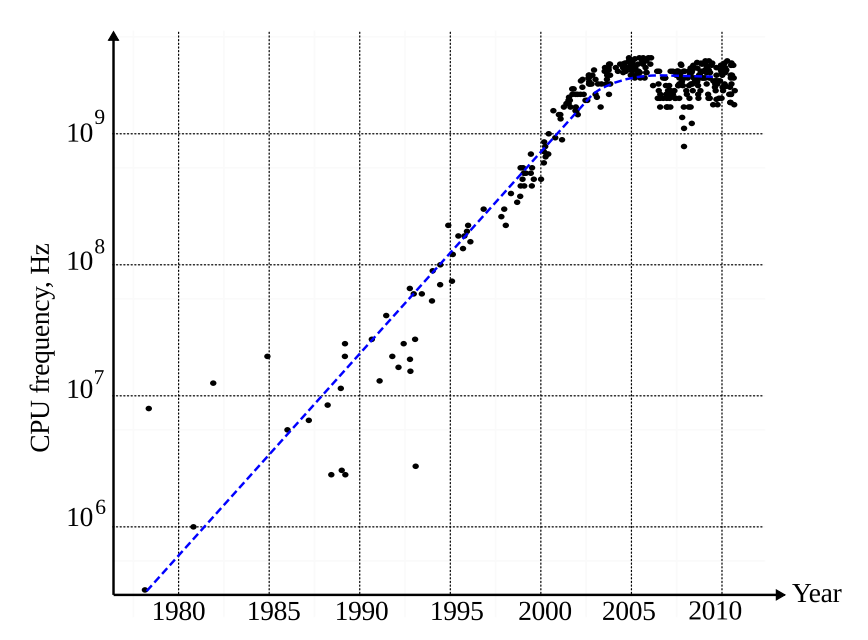
\includegraphics[scale=0.4]{../eldar_last_30_yrs}
	\caption{Frequency of the Intel microprocessors over past 30 years \cite{zianbetov2013phd}.}
	\label{fig:eldar_last_30_yrs}
\end{figure}\\
This plateauing of clock frequency has been caused by high power consumption due to the demands placed by the global distribution of a high frequency clock, often the single biggest consumer of power on the chip \cite{tiwari1998reducing}.
With the growth of the \ac{IOT} market where low power devices are desirable, with many of the emerging uses of \ac{SOC}s being portable and thus without a permanent power source, high power consumption goes directly against one of the key pillars of the technology. This forces many of these devices to use lower performance hardware in order to reduce the power consumption, and increase the battery life, of their devices.

In digital systems, two main approaches are used when designing the clocking system. In both cases, the chip is broken down into small areas in which all transistors are clocked synchronously, with the size constrained by the ability to deliver a quality clock signal to all transistors. The first of these methods is \ac{GSLS}, where the clock signals in each of these subregions of the chip are synchronised with one other. In practice, however, this is very difficult to achieve, as extremely high precision is required across the ever increasing number of transistors and the entire area of the chip, and doing so leads to high power consumption.

In contrast in a \ac{GALS} clock delivery system the ``local'' areas are not synchronised with other. This reduces the clocking system's complexity and thus the power consumption and chip area used, at the expense of communication speed between blocks. This disadvantage comes from the need to then somehow synchronise the messages being sent from one area to another to avoid the corruption of any messages.
A \ac{GSLS}, system, however has the advantages of deterministic behaviour and greater rates of communication between clocking areas and, as such, remains a desirable system design. A number of methods which deliver \ac{GSLS} clocking exist at present such as clock trees as well as emerging technologies such as ADPLL networks.

\section{The Impact of Clocking Errors}
In Figure \ref{fig:eldar_why_precise_clocking} the data path between two synchronously clocked registers is shown, with the circuit's function being carried out by the combinatorial network between the registers.
Each register has a setup time, which represents the amount of time that the input value to a register must remain constant before the clock edge, and a hold time, the time for which the input must remain constant after a clock edge.
\begin{figure}[h]
	\centering
	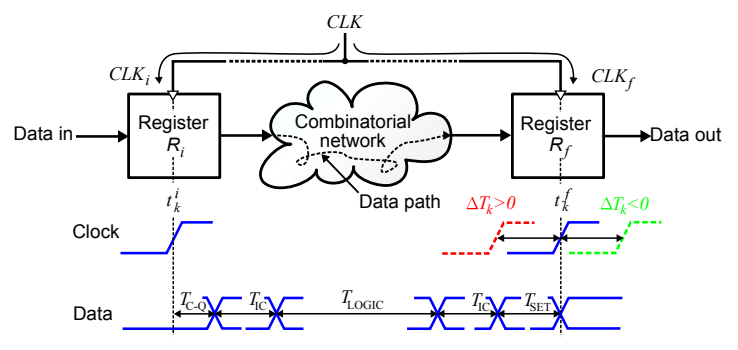
\includegraphics[scale=0.6]{../eldar_why_precise_clocking}
	\caption{Data Flow in a Clocked System \cite{zianbetov2013phd}.}
	\label{fig:eldar_why_precise_clocking}
\end{figure}

A lack of synchronisation between the clock edges will manifest itself as a time difference between the clocking events at both registers, $\Delta T = t^i_k - t^f_k$. $\Delta T$ is considered to be ergodic and can be described by an average deviation called skew and random process, normally modelled as a Gaussian random variable. If $\Delta T$ is negative this reduces the time available for the intervening combinatorial network thereby, having the same effect as a reduction in clocking frequency. Correspondingly a positive $\Delta T$ for depicted registers implies a negative $\Delta T$ for $R_f$ and the subsequent register. 
The most common sources of clock error are caused by mismatches which usually stem from production, such as differences in the length of clocking paths, buffer delays or in the parameters of either active or passive components in the clock distribution network, which as the size of components on an \ac{IC} reduces becomes more difficult to avoid. All sources of mismatch will manifest themselves in the clock distribution system as skew between transistors, while the noise in active components or the power supply system will appear as jitter in the clock signal.

\section{Traditional Solutions}
A number of traditional solutions exist which provide \ac{GSLS} clocking systems, using a variety of techniques. The most simple of these implement clock distribution systems that are symmetrical in order to distribute a centrally generated clock signal to all areas of the chip at the same phase. These systems are named in accordance with their geometry, with the most common variants being branch, X or H trees. 
\begin{figure}[h]
	\centering
	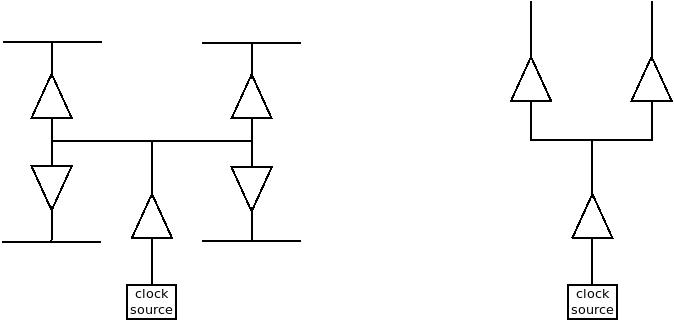
\includegraphics[scale=0.33]{../trees}
	\caption{H and Branch Tree Clock Distribution Systems.}
	\label{fig:trees}
\end{figure}

While on the surface these appear simple, the task of obtaining an exact matching is, in practice, the limiting factor in this design. Even if the clock distribution system is geometrically symmetrical by design, production mismatches in either active or passive components will lead to a skew that varies from part to part. In order to minimise the impact of production tolerances, the dimensions of components in the distribution network can be increased, thus reducing the relative variation possible. However this has the impact of increasing the power consumption of the distribution network \cite{tiwari1998reducing}.

A mesh clock distribution network is an alternate design where the clock is delivered using a Cartesian grid of distribution lines. Compared to a tree type system, the variation in skew seen with a clock mesh is inversely proportional to the density of the grid while the sources of jitter remain identical. According to Abdelhadi \textit{et al} (2010) clock meshes ``\textit{achieve low and deterministic skew, low skew variations, and low jitter}'', all desirable characteristics for a clock distribution system. However they dissipate more power due to extra capacitive loading, attributable to vast number of lines required to form the grid. Similarly mesh distribution networks suffer from potential mismatch in production and alleviation through increasing of the dimensions of interconnects will, as with a tree type system, lead to higher power consumption \cite{abdelhadi2010timing}. 
\begin{figure}[h]
	\centering
	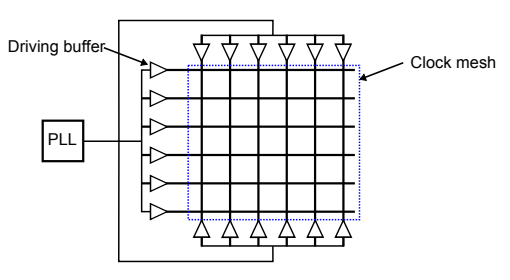
\includegraphics[scale=0.7]{../tex_files/eldar_mesh}
	\caption{Mesh Clock Distribution System \cite{zianbetov2013phd}.}
	\label{fig:mesh}
\end{figure}
Alternative designs replace the electrical lines used in the tree networks with waveguides for optical signals, with only the distribution in the local area carried out using regular wires. This technique presents many advantages \cite{chen2006chip}: optical clock delivery is immune to the noise sources that affect electrical clock distribution systems, consume less power and do not suffer from the electrical losses present in a regular tree system.

\section{Skew Compensation}
In a tree type distribution system, skew is the main issue affecting clock accuracy and as such some effort has gone into addressing the problem. Skew due to the manufacturing process can be, at least, partly accounted for by means of active control through a skew compensator. This is a circuit, or controller, that compares the skew of each local clocking area on the chip and attempts to ensure in-phase clock delivery. Two main strategies exist to provide skew compensation, each named according to the location of the control mechanism. Designs featuring the controller located at the clock source, are known as ``centralised'' methods, and those with multiple controllers in the individual clocking areas known as ``decentralised''. Regardless of the controller placement these techniques allow for the tuning of the propagation delay between the centralised clock source and the local clocking areas.

In a centralised skew compensation circuit, the skew across the chip is calculated by the central controller which then manipulates the distribution network in order to deliver a more in-phase clock around the chip. This calculation is done by measuring the round trip time from the clock source to both the root of local clock tree, and to the individual ``leaves'' of the tree. The controller then has a limited ability to tune the propagation path. The downsides of this technique are the resolution of both the measurement and compensation are poor, allowing for the correction of just skew and not of any jitter that may be present in the system, and that the extra circuitry required for both the tunability of the forward path and the two extra return paths contribute to an increased footprint and power consumption.

As the name suggest a decentralised skew compensation technique delegates the responsibility of tuning the propagation path to the individual clock regions. This strategy has the advantage of not requiring the return paths present in a ``centralised'' design. Instead comparison is made betweeen the leaves of different clocking areas and on this basis the propagation delay is varied.
For example, Yamashita \textit{et al} (2005) designed a system in which each clocking area or ``leaf node'' contains a partial clock tree. Each of these ``leaves'' is able to compare its clock phase to the neighbouring node, and based on the result, tune an adjustable delay buffer \cite{yamashita2005dynamic}. While this method can compensate for process, voltage and temperature variation, it does not address the power consumption due to the delivery of a high frequency clock across the entire chip area nor does it have any impact on clock jitter.

%DOWN TO HERE DONE FOR ACRO
\section{Multi-oscillator Designs}
The designs described previously, are all similar in that they have a single central oscillator that provides the clock for all areas of the chip, whereas the following methods attempt to synchronise multiple oscillators, each of which provides the clock for a single clocking area. The main advantage of a multi-oscillator design, is that as each clocking area has its clock created locally, there is no problem with signal degradation. Similar to a decentralised skew compensation scheme comparisons are only made to neighbouring blocks and as such there is reduced power loss due to transmission.
\begin{figure}[h]
	\centering
	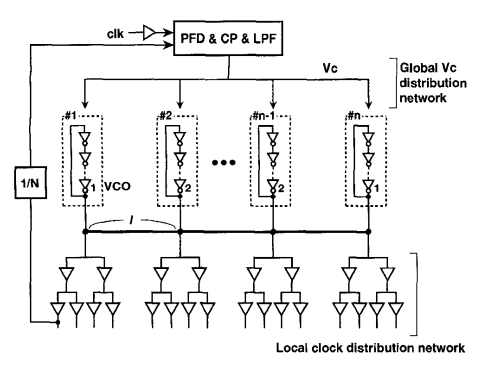
\includegraphics[scale=0.7]{../mizuno1998noise}
	\caption{Coupled Oscillator Clock Delivery Circuit \cite{mizuno1998noise}.}
	\label{fig:mizuno1998noise}
\end{figure}
One such method is a network of oscillators as in Figure \ref{fig:mizuno1998noise} which uses coupled PLLs to generate local clocks. The advantage of this method is that only the control voltage $v_c$ needs delivery to all areas of the chip, thus alleviating the need for a power hungry distribution circuit, while also being more noise-immune than the transmission of a high frequency clock. However this design still suffers from clock variation as all VCOs are fed the same control voltage, and this is acknowledged by the authors:
\begin{quotation}
	\textit{Unfortunately, as with the conventional ... method, distributing the VCOs over the entire chip causes the problem that jitter and skew are increased by variations in the fabrication process (static), temperature, and power supply (dynamic)} \cite{mizuno1998noise}.
\end{quotation}
This design also only compares the phase of a single branch of the distribution network with the reference, in order calculate the control voltage which again may contribute to a degradation in clock synchronisation. %TODO why

Another potential multi-oscillator design synchronises the oscillators using the phase relationship with the oscillators in the neighbouring clocking area. Once again, this negates the requirement for a global distribution structure and comparisons need only be made with neighbouring areas. As a phase lock loop is being used only a divided down version of the clock is required. This in turn means the hardware transporting the divided clock signal to the phase comparator, has significantly lower requirements placed on it, thus lowering the power consumption. Pratt and Nguyen initially proposed this design in their paper published in 1995 entitled ``\textit{Distributed Synchronous Clocking}'' in which they propose a Cartesian grid of clocking areas, each with their own PLL, which has become known as a PLL Network \cite{pratt1995distributed}. In this design any given node is synchronised with its neighbours and one of the corner nodes is additionally synchronised with the reference. According to the authors this is ``a simple, effective way to achieve low cost, high quality, low skew clock generation in a synchronous parallel processor''. This methodology was implemented by Gutnik \textit{et al} (2000) who found:
\begin{quote}
	\textit{Design and measurements on this chip confirm that generating and synchronizing multiple clocks on chip is feasible. Neither the power nor the area overhead of multiple PLLs is substantial compared to the cost of distributing the clock by conventional means} \cite{gutnik2000active}.
\end{quote}
\begin{figure}[h]
	\centering
	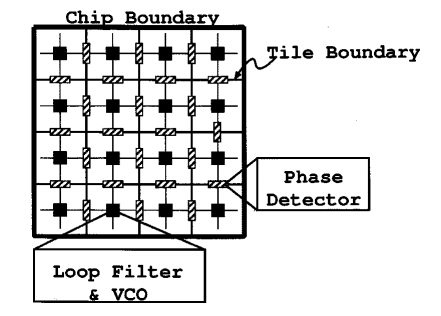
\includegraphics[scale=0.7]{../gutnik2000active}
	\caption{PLL Network Topology \cite{gutnik2000active}.}
	\label{fig:gutnik2000active}
\end{figure}

\section{ADPLL Networks}
As a PLL network is an analog circuit, its integration in a modern IC is a barrier to usage and it has not been used in any commercial designs \cite{zianbetov2013distributed}. An alternative design that is more suitable for current fabrication techniques eschews from using analog components and instead implements the network of controlled oscillators using only digital circuitry, hence the name All-Digital PLL. A 4x4 ADPLL network was designed and prototyped in 65 nm CMOS by Zianbetov and Shan in order to test the suitability of the technique as a clock distributor \cite{zianbetov2013phd,shan2014phd}. %TODO fix phd references

In this design the oscillators are coupled using digital phase comparators which attempt to measure the phase error between two oscillators with each non edge node being connected to four neighbours. Figure \ref{fig:eldar_node} shows high level detail of the architecture of both the entire clocking system and that of an individual node in the design. A digital PLL network has the additional advantages over its analog counterparts that it can benefit from advancements in digital circuit design suites, be reconfigurable and programmable and has a significantly greater immunity to perturbations inherent to its digital nature \cite{zianbetov2013phd}. This last advantage is of particular use in a digital environment, as otherwise there is potential for clock degradation resulting from switching of transistors.
\begin{figure}[h]
	\centering
	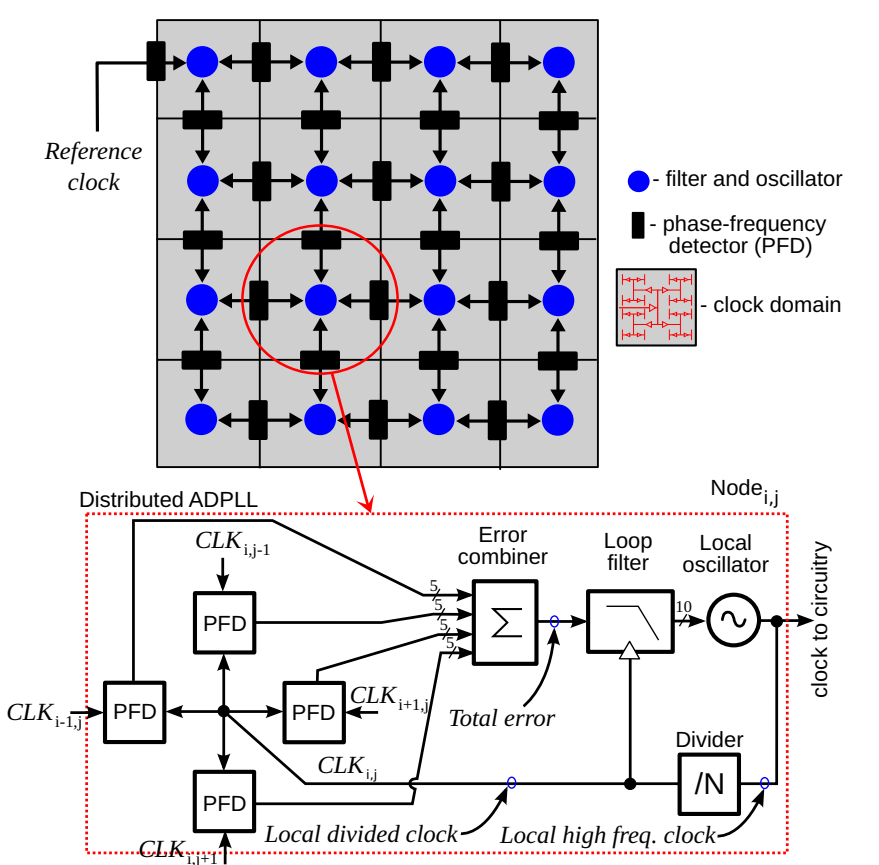
\includegraphics[scale=0.4]{../ccirc_2013_arch}
	\caption{Architecture of the ADPLL network and of a single node \cite{zianbetov2013distributed}.}
	\label{fig:eldar_node}
\end{figure}
Looking at the design of a given node it is notable that the function carried out by the Error Combiner is akin to a average, therefore as mentioned by Pratt and Nyugen, there is potential to settle in a stable ``mode'' in which the oscillators are not synchronised. In their paper, they present a method where initial start-up is performed uni-directionally and, once all nodes are close to alignment, full connectivity can be restored, however this was not viable in an analog system \cite{pratt1995distributed}. In creating an entirely digital system, Zianbetov and Shan could exploit the reconfigurability and and implement this system at start-up.

\section{ADPLL Architecture}
As indicated in Figure \ref{fig:mulkeen_pll} the three main building blocks of a conventional Phase Lock Loop are the Phase Detector, Loop Filter and Controllable Oscillator. In the All-Digital counterpart each of these traditionally analog components are replaced by their digital counterparts, necessitating quantisation in order to remain physically realisable. 
\begin{figure}[h]
	\centering
	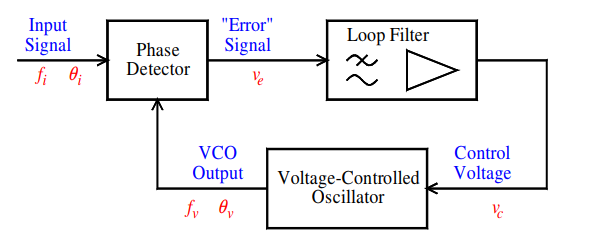
\includegraphics[scale=0.5]{../tex_files/mulkeen_pll}
	\caption{Block Diagram of a Phase Lock Loop, \textit{Wireless Systems Notes}, B. Mulkeen (2017).}
	\label{fig:mulkeen_pll}
\end{figure}